%% Figure from MATH 556 notes, section 43 (Lecture 18). ADDED (not from lecture).
\begin{tikzpicture}[>=stealth]
  \begin{scope}[xshift=0cm, xscale=0.62, yscale=1.1]
    \begin{scope}\clip (0,0) rectangle (6.2832,1.05); \fill[blue!25] (0,0) -- plot[domain=0:6.2832, samples=400] (\x,{\x/(2*pi)*sin(2*\x r)}) -- (6.2832,0) -- cycle; \end{scope}
    \begin{scope}\clip (0,-1.05) rectangle (6.2832,0); \fill[red!25] (0,0) -- plot[domain=0:6.2832, samples=400] (\x,{\x/(2*pi)*sin(2*\x r)}) -- (6.2832,0) -- cycle; \end{scope}
    \draw[gray, dashed] plot[domain=0:6.2832, samples=2] (\x,{\x/(2*pi)}); \draw[gray, dashed] plot[domain=0:6.2832, samples=2] (\x,{-\x/(2*pi)});
    \draw[->] (0,0) -- (6.7,0); \draw (0,-1.05) -- (0,1.05);
    \draw[thick, black!80] plot[domain=0:6.2832, samples=400] (\x,{\x/(2*pi)*sin(2*\x r)});
    \node[font=\small] at (3.1416,1.35) {$m = 2$};
    \node[font=\scriptsize] at (3.1416,-1.35) {$\int_0^{2\pi} g \sin(mx)\, dx = -\tfrac{1}{2}$};
  \end{scope}
  \begin{scope}[xshift=4.9cm, xscale=0.62, yscale=1.1]
    \begin{scope}\clip (0,0) rectangle (6.2832,1.05); \fill[blue!25] (0,0) -- plot[domain=0:6.2832, samples=400] (\x,{\x/(2*pi)*sin(6*\x r)}) -- (6.2832,0) -- cycle; \end{scope}
    \begin{scope}\clip (0,-1.05) rectangle (6.2832,0); \fill[red!25] (0,0) -- plot[domain=0:6.2832, samples=400] (\x,{\x/(2*pi)*sin(6*\x r)}) -- (6.2832,0) -- cycle; \end{scope}
    \draw[gray, dashed] plot[domain=0:6.2832, samples=2] (\x,{\x/(2*pi)}); \draw[gray, dashed] plot[domain=0:6.2832, samples=2] (\x,{-\x/(2*pi)});
    \draw[->] (0,0) -- (6.7,0); \draw (0,-1.05) -- (0,1.05);
    \draw[thick, black!80] plot[domain=0:6.2832, samples=400] (\x,{\x/(2*pi)*sin(6*\x r)});
    \node[font=\small] at (3.1416,1.35) {$m = 6$};
    \node[font=\scriptsize] at (3.1416,-1.35) {$\int_0^{2\pi} g \sin(mx)\, dx = -\tfrac{1}{6}$};
  \end{scope}
  \begin{scope}[xshift=9.8cm, xscale=0.62, yscale=1.1]
    \begin{scope}\clip (0,0) rectangle (6.2832,1.05); \fill[blue!25] (0,0) -- plot[domain=0:6.2832, samples=400] (\x,{\x/(2*pi)*sin(18*\x r)}) -- (6.2832,0) -- cycle; \end{scope}
    \begin{scope}\clip (0,-1.05) rectangle (6.2832,0); \fill[red!25] (0,0) -- plot[domain=0:6.2832, samples=400] (\x,{\x/(2*pi)*sin(18*\x r)}) -- (6.2832,0) -- cycle; \end{scope}
    \draw[gray, dashed] plot[domain=0:6.2832, samples=2] (\x,{\x/(2*pi)}); \draw[gray, dashed] plot[domain=0:6.2832, samples=2] (\x,{-\x/(2*pi)});
    \draw[->] (0,0) -- (6.7,0); \draw (0,-1.05) -- (0,1.05);
    \draw[thick, black!80] plot[domain=0:6.2832, samples=400] (\x,{\x/(2*pi)*sin(18*\x r)});
    \node[font=\small] at (3.1416,1.35) {$m = 18$};
    \node[font=\scriptsize] at (3.1416,-1.35) {$\int_0^{2\pi} g \sin(mx)\, dx = -\tfrac{1}{18}$};
  \end{scope}
\end{tikzpicture}
